\documentclass{standalone}
\usepackage{tikz}
\usetikzlibrary{shapes}
\begin{document}
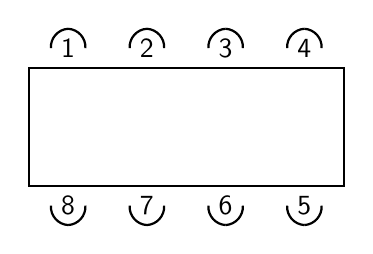
\begin{tikzpicture}[thick, every node/.style = {font = \sffamily}]
\draw (-.5,.25) rectangle (3.5,1.75);
\node (8) at (0,0) {8};
\node (7) at (1,0) {7};
\node (6) at (2,0) {6};
\node (5) at (3,0) {5};
\node (1) at (0,2) {1};
\node (2) at (1,2) {2};
\node (3) at (2,2) {3};
\node (4) at (3,2) {4};
\foreach \i in {8,7,6,5} {
	\draw (\i.west) to [bend right = 45] (\i.south);
	\draw (\i.south) to [bend right = 45] (\i.east);
};
\foreach \i in {1,2,3,4} {
	\draw (\i.east) to [bend right = 45] (\i.north);
	\draw (\i.north) to [bend right = 45] (\i.west);
};
\end{tikzpicture}
\end{document}
